\section{Séance 6 et 7}

\begin{exo}
Soient $A$ et $B$ deux ensembles finis avec $|A|=a$ et $|B|=b$ ($a,b \in \mathbb{N}$). Que valent:
\begin{enumerate}[(i)]
\item $|A\times B|$,
\item $|B^A|$ o\`u $B^A:=\{f:A \rightarrow B\}$,
\item $|\{f:A \rightarrow B: f \mathrm{~est~une~injection~de~} A \mathrm{~dans~}B\}|$,
\item $|\mathrm{Sym}\,A|$ o\`u $\mathrm{Sym}\,A$ est l'ensemble des permutations de $A$.
\end{enumerate}
\end{exo}

\begin{enumerate}[(i)]
	\item $a\cdot b$
	\item $b^a$
	\item Si $\#B < \#A$ pas d'injection possible, donc vaut zéro. Sinon, $(b-a+1)\cdot ... \cdot (b-a) \cdot b$ = $ \frac{b!}{(b-a)!}$
	\item $a!$
\end{enumerate}

%----------------------------------------------

\begin{exo}
Quels sont les ensembles $F$ non vides ayant la propri\'et\'e suivante:
\begin{enumerate}[(i)]
\item pour tout ensemble $X$, $|F^X|=1$?
\item pour tout ensemble $Y$, $|Y^F|=1$?
\end{enumerate}
\end{exo}

\begin{enumerate}[(i)]
	\item $|F| = 1 $
	\item Ensemble vide (mais pas possible par énoncé)
\end{enumerate}

%----------------------------------------------

\begin{exo}
Soient $f:A \rightarrow B$ et $g:B \rightarrow C$ deux fonctions. D\'emontrer:
\begin{enumerate}[(i)]
\item $g \circ f$ injective $\Rightarrow$ $f$ injective;
\item $g \circ f$ surjective $\Rightarrow$ $g$ surjective;
\item $g \circ f$ bijective $\Rightarrow$ ($f$ injective et $g$ surjective).
\end{enumerate}
\end{exo}

\begin{enumerate}[(i)]
	\item Si f non injective, deux éléments $a_{1}$ et $a_{2}$ différents de A vont être envoyés par f sur un élément b de B. De plus, ces deux éléments vont être envoyés par g o f sur un même élément c de C, car g ( f ($a_1$)) = g( b ) = c = g( b) = g ( f ( $a_2$))
	\item On sait que $\forall c \in C , \exists a \in A$ tel que g o f (a) = c. 
		On veut montrer que g est surjective. C'est à dire que $\forall c \in C, \exists b \in B$ tel que g (b) = c. 
		Ceci est vérifié en prenant b = f(a).
	\item Implication de (i) et (ii)
\end{enumerate}

%----------------------------------------------

\begin{exo}
Donner une preuve bijective de l'identit\'e de somme parall\`ele ${k \choose k} + {k+1 \choose k} + \cdots + {m \choose k} = {m+1 \choose k+1}$.
\end{exo}

Voir syllabus année passée page 8.

%----------------------------------------------

\begin{exo}
Donner deux d\'emonstrations de
$$
\sum_{k=0}^n {n \choose k} = 2^n\ .
$$
\end{exo}

Première démonstration: 

Via le Binôme de Newton, on sait que

$$(x+y)^n = \sum_{k=0}^n {n \choose k} x^{n-k} y^k$$

Si on pose x=1 et y=1, on a: 

\begin{align*}
 (1+1)^n &= \sum_{k=0}^n {n \choose k} \cdot \underbrace{1^{n-k}}_{=1} \cdot \underbrace{1^k}_{=1} 
 2^n &= \sum_{k=0}^n {n \choose k}
\end{align*}

Deuxième démonstration: 

${n \choose k}$ est le nombre de sous-ensembles à k éléments d'un ensemble à n éléments. 

$$ |\{ 0,1 \}^n| = 2^n $$

%----------------------------------------------

\begin{exo}
Qu'obtient-on comme identit\'e sur les coefficients binomiaux en \'ecrivant
$$
(x+y)^{2n} = (x+y)^n(x+y)^n\ ?
$$
\end{exo}

(Voir avec assistants)

%----------------------------------------------

\begin{exo}
Qu'obtient-on en d\'erivant la formule du bin\^ome~?
\end{exo}

(Voir avec assistants)

%----------------------------------------------

\begin{exo}
Trouver le nombre de solutions de l'\'equation $x + y + z + w = 15$, dans les naturels.
\end{exo}

$ { s + d - 1 \choose d - 1 } = { 15 + 4 - 1 \choose 4 - 1} = {18 \choose 3 }$

%----------------------------------------------

\begin{exo} 
Combien l'\'equation
$$
x + y + z + t + u = 60
$$
poss\`ede-t-elle de solutions enti\`eres $(x,y,z,t,u)$ telles que
$$
x > 0\ ,\quad y \geqslant 9\ , \quad z > -2\ , \quad t \geqslant 0 \quad \textrm{ et }  \quad u > 10 \quad ?
$$
\end{exo}

On doit procéder à un changement de variables.

${x}' = x-1 \Leftrightarrow x= {x}'+1 \qquad {y}' = y-9 \Leftrightarrow y= {y}'+9 \qquad {z}' = z+1 \Leftrightarrow z= {z}'-1 $

$\qquad \qquad \qquad \qquad \qquad {t}' = t \qquad {u}' = u-11 \Leftrightarrow u= {u}'+11$

${x}'+{y}'+{z}'+{t}'+{u}' = 60 - 1 - 9 + 1 - 11 = 40$

${s + d - 1 \choose d - 1} = {40 + 5 - 1 \choose 5 - 1} = {44 \choose 4}$
%----------------------------------------------

\begin{exo} 
Trouver le nombre de solutions de l'in\'equation
$$
x + y + z + t \leqslant 6
$$
%
\begin{enumerate}[(i)]
\item dans les naturels;
\item dans les entiers $>0$;
\item dans les entiers, avec comme contraintes suppl\'ementaires $x > 2$, $y > -2$, $z > 0$ et $t > -3$.
\end{enumerate}
\end{exo}

Même chose que les exos précédents (réponse dans un prochain épisode...).

%----------------------------------------------

\begin{exo} 
Avec les lettres du mot MISSISSIPPI, combien peut-on \'ecrire de mots diff\'erents de 11 lettres~?
\end{exo}

Lettres du mot: 1 M, 4 I, 4 S, 2 P 

Mots de 11 lettres: $ \frac{11!}{(4!)(4!)(2!)(1!)}$

%----------------------------------------------

\begin{exo} 
Avec les lettres du mot 
%
\begin{center}
H\,U\,M\,U\,H\,U\,M\,U\,N\,U\,K\,U\,N\,U\,K\,U\,A\,P\,U\,A\,A
\end{center}
(``poisson'' en hawa\"\i{}en), combien peut-on \'ecrire de mots diff\'erents de 21 lettres ne comprenant pas deux lettres U c\^ote \`a c\^ote~?
\end{exo}

Faire mots de 12 lettres sans U. Rajouter probabilité de mettre les U dans les 13 places qui restent pour faire des mots de 21 lettres. Donc, ${13 \choose 9}$

%----------------------------------------------

\begin{exo} 
Si $0 \leqslant m \leqslant n$, que vaut
$$
\sum_{k=m}^n {k \choose m}{n \choose k}\quad ?
$$
(Hint~: essayer une preuve bijective.)
\end{exo}

Preuve version "étudiant": 

\begin{align*}
 \sum_{k=m}^n {k \choose m}{n \choose k} &= \sum_{k=m}^n \frac{\cancel{k!}}{m!(k-m)!} \frac{n!}{\cancel{k!}(n-k)!} = \sum_{k=m}^n \frac{n!}{m!(k-m)!(n-k)!} 
 &= \sum_{k=m}^n \frac{n!}{m!(k-m)!(n-k)!} \frac{(n-m)!}{(n-m)!} = {n \choose m} \sum_{k=m}^n \frac{(n-m)!}{(k-m)!(n-k)!} 
 &= {n \choose m} \sum_{k=m}^n {n-m \choose k-m} \vspace{1cm} \qquad \text{On pose} \quad r=k-m 
 &= {n \choose m} \sum_{r=0}^{n-m} {n-m \choose r} 1^{r} 1^{n-m-r} \qquad \text{Formule du binôme de Newton} 
 &= {n \choose m} (1+1)^{n-m} = {n \choose m} 2^{n-m} 
\end{align*}

Preuve bijective version assistants: 

\begin{minipage}{0.4\textwidth}
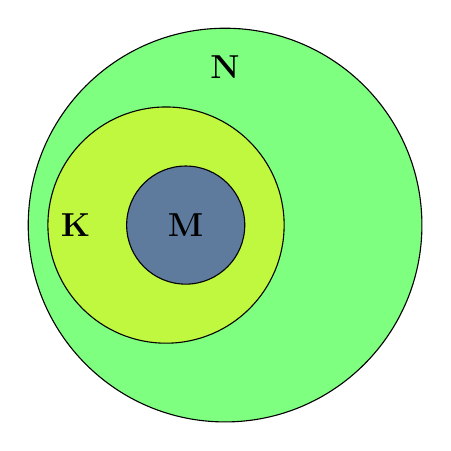
\begin{tikzpicture}[scale=0.5]

\begin{scope}[shift={(3cm,-5cm)}, fill opacity=0.5,
  mytext/.style={text opacity=1,font=\large\bfseries}]

\draw[fill=green, draw = black] (0,0) circle (5);
\draw[fill=yellow, draw = black] (-1.5,0) circle (3);
\draw[fill=blue, draw = black] (-1,0) circle (1.5);

\node[mytext] at (0,4) (N) {N};
\node[mytext] at (-3.8,0) (K) {K};
\node[mytext] at (-1,0) (M) {M};
\end{scope}
\end{tikzpicture}
\end{minipage}
\begin{minipage}{0.6\textwidth}
Fixons $0 \leq m \leq n$
Comptons de 2 manières différentes le nombre de triples (M, K, N) où $M \subseteq K \subseteq N$ et |M| = m, |N| = n, |K| = k

\begin{enumerate}
\item On choisit un ensemble de taille m dans N: il y a ${n \choose m}$ façons de choisir
\item K peut avoir m éléments, m+1, ..., n éléments 
\end{enumerate}
\end{minipage}

\vspace{1cm}

\textbf{1. On choisit un ensemble de taille m dans N: il y a ${n \choose m}$ façons de choisir}

Ensuite, nous complétons cet ensemble M pour obtenir K, c'est à dire il y a $$\sum_{k=0}^{n-m} {n-m \choose k} = 2^{n-m} \quad \text{choix}$$ 

Donc au total il y a ${n \choose m} 2^{n-m}$ choix.

\textbf{2. K peut avoir m éléments, m+1, ..., n éléments} 

\begin{enumerate}
\item \textbf{S'il y en a m:} on choisit m éléments parmi n et m éléments parmi ces m éléments, c'est à dire ${m \choose m}{n \choose m}$
\item \textbf{S'il y en a m+1:} on choisit m+1 éléments parmi n et m éléments parmi ces m+1 éléments, c'est à dire ${m+1 \choose m}{n \choose m+1}$
\item \textbf{S'il y en a n:} on choisit n éléments parmi n et m éléments parmi ces n éléments, c'est à dire ${n \choose m}{n \choose n}$ 
\end{enumerate}

Il suffit de tout sommer (car "ou exclusif"). Donc: $$ \sum_{k=m}^n {k \choose m}{n \choose k} = {n \choose m} 2^{(n-m)}$$

\vspace{1cm}

%----------------------------------------------

\begin{exo} 
Si on jette simultan\'ement $n$ d\`es identiques, combien de r\'esultats diff\'erents peut-on obtenir~? (Deux r\'esultats sont consid\'er\'es comme \'equivalents s'ils ont le m\^eme nombre de 1, le m\^eme nombre de 2, \ldots, le m\^eme nombre de 6.)
\end{exo}

(Voir avec assistants)